\chapter{Part 1\  论文回顾}

\begin{figure}[H]
	\centering
	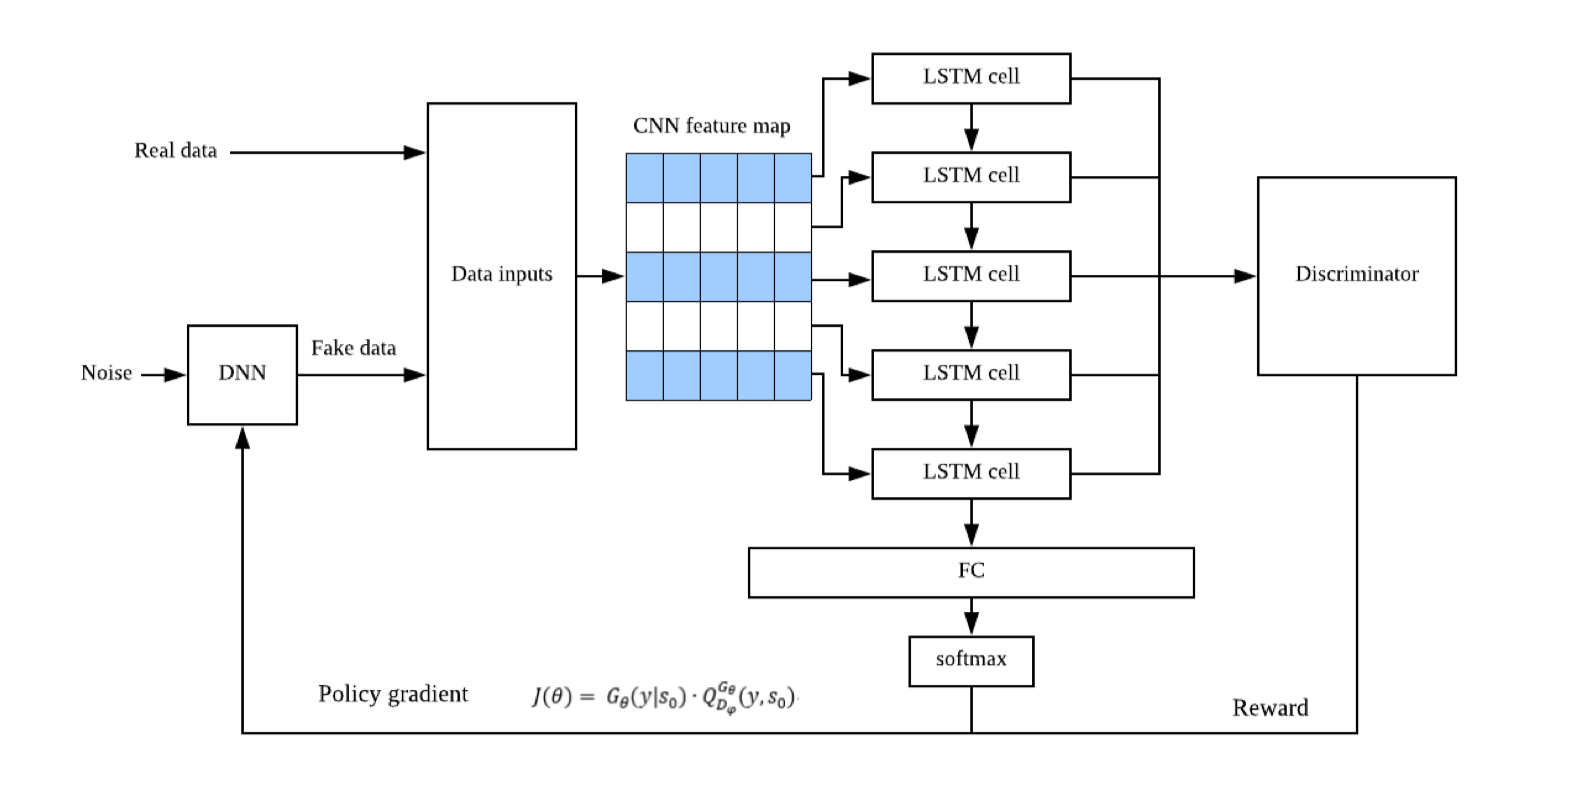
\includegraphics[width = 1.2\columnwidth]{InmemoryDatabaseExperiment/fig/img17.jpg}
	\caption{模型架构}
\end{figure}

\section{C-LSTM}
\paragraph{C-LSTM在本文中的作用}
\begin{itemize}
    \item 可以分辨是生成的数据还是自然的数据
    \item 识别正常数据
\end{itemize}
\paragraph{C-LSTM可以提取时间和空间信息,相比于传统的CNN或者LSTM提取的信息层次更丰富}
\paragraph{接受生成器生成的数据,打出一个score,作为属于哪一类别等分数,与Discriminator的Reward结合在一起,实行Policy gradient}
\paragraph{改进}
\begin{itemize}
    \item 只用最后一个LSTM cell的输出作为Discriminator的输入
\end{itemize}

\section{GAN}
\paragraph{本文的目的是用于生成异常数据,是连续的,所以不用蒙特卡罗搜索}




\chapter{Part 2\  工作设想}

\paragraph{先用分别用C-LSTM和GAN进行异常检测实验}
\begin{itemize}
    \item 划窗的size如何确定和优化
    \item oversampling with VAE
\end{itemize}



\chapter{Appendix A}
\listoffigures

% \chapter{Appendix B}
% \listoftables
